\section{RESULTS AND DISCUSSION}
\begin{figure}[th!]
\subfigure[One fluid solve per iteration.]{
    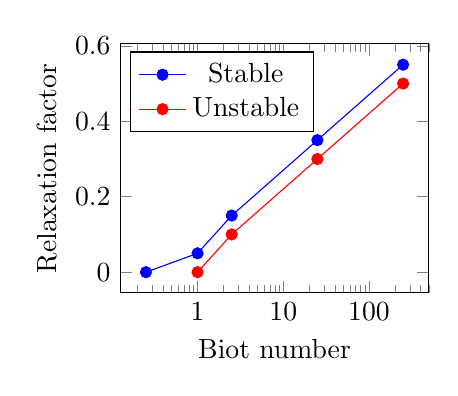
\begin{tikzpicture}
\begin{semilogxaxis}[width=55mm,
	%title={FFTB stability},
	legend pos=north west,
    unbounded coords=discard,
    log basis x=10,
    log ticks with fixed point
    ,xlabel=Biot number,ylabel=Relaxation factor]
\addplot[blue, mark=*] coordinates {
(0.25,
0.00)
(1,
0.05)
(2.5,
0.15)
(25,
0.35)
(250,
0.55)
};
\addplot[red, mark=*]  coordinates {
(1,
0.00)
(2.5,
0.10)
(25,
0.30)
(250,
0.50)
};
\legend{Stable,Unstable}
\end{semilogxaxis}
\end{tikzpicture}
    \label{fig:subfig1}
}
\subfigure[Ten fluid solves per iteration.]{
    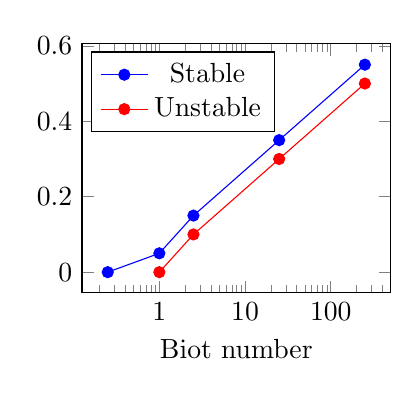
\begin{tikzpicture}
\begin{semilogxaxis}[width=55mm,
	%title={FFTB stability},
	legend pos=north west,
    unbounded coords=discard,
    log basis x=10,
    log ticks with fixed point
    ,xlabel=Biot number,ylabel=]
\addplot[blue, mark=*] coordinates {
(0.25,
0.00)
(1,
0.05)
(2.5,
0.15)
(25,
0.35)
(250,
0.55)
};
\addplot[red, mark=*]  coordinates {
(1,
0.00)
(2.5,
0.10)
(25,
0.30)
(250,
0.50)
};
\legend{Stable,Unstable}
\end{semilogxaxis}
\end{tikzpicture}
    \label{fig:subfig2}
}
\subfigure[100 fluid solves per iteration.]{
    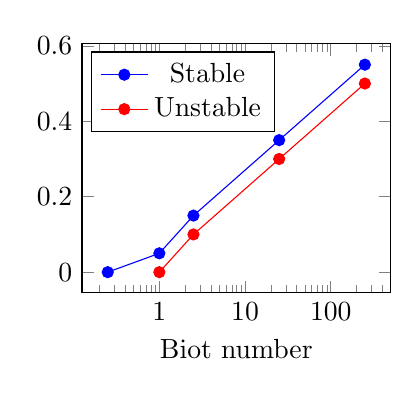
\begin{tikzpicture}
\begin{semilogxaxis}[width=55mm,
	%title={FFTB stability},
	legend pos=north west,
    unbounded coords=discard,
    log basis x=10,
    log ticks with fixed point
    ,xlabel=Biot number,ylabel=]
\addplot[blue, mark=*] coordinates {
(0.25,
0.00)
(1,
0.05)
(2.5,
0.15)
(25,
0.35)
(250,
0.55)
};
\addplot[red, mark=*]  coordinates {
(1,
0.00)
(2.5,
0.10)
(25,
0.30)
(250,
0.50)
};
\legend{Stable,Unstable}
\end{semilogxaxis}
\end{tikzpicture}
    \label{fig:subfig3}
}
  \caption{Stability of the FFTB method as a function of the Biot number for different fluid solves per iteration.}
\end{figure}